
\noindent \textbf{L2.2 (Sipser 1.6c)} Dê um DFA/AFD para $A = \{w \ |\ w$ possui $0101$ por subcadeia\}. Considere o alfabeto $\Sigma = \{0, 1\}$.\\[3pt]
\textbf{Resposta: } Para este exercício, utilizei as referências em \cite{illinois3}, \cite{illinois2} e \cite{hopcroft2006}.

Seja $M = \{Q, \Sigma, \delta, s, F\}$ o AFD da figura \ref{fig:sip1.6c} que reconhece $A$, onde:
\begin{enumerate}[label=\textbf{\arabic*}]
    \item $Q = \{q_0, q_1, q_2, q_3, q_4\}$
    \item $\Sigma = \{0, 1\}$
    \item $\delta = $
        \begin{table}[!ht]
        \centering
        \rot{\hspace{5 mm}\llap{Estados}}
        \begin{tabular}{l|l|l}
                & 0         & 1     \\ \hline
        $q_0$   & $q_1$     & $q_0$ \\
        $q_1$   & $q_1$     & $q_2$ \\
        $q_2$   & $q_3$     & $q_0$ \\
        $q_3$   & $q_1$     & $q_4$ \\
        $q_4$   & $q_4$     & $q_4$
        \end{tabular}
        \end{table}
    \item $s = q_0$
    \item $F = \{q_4\}$
\end{enumerate}

\begin{figure}[H]
\centering
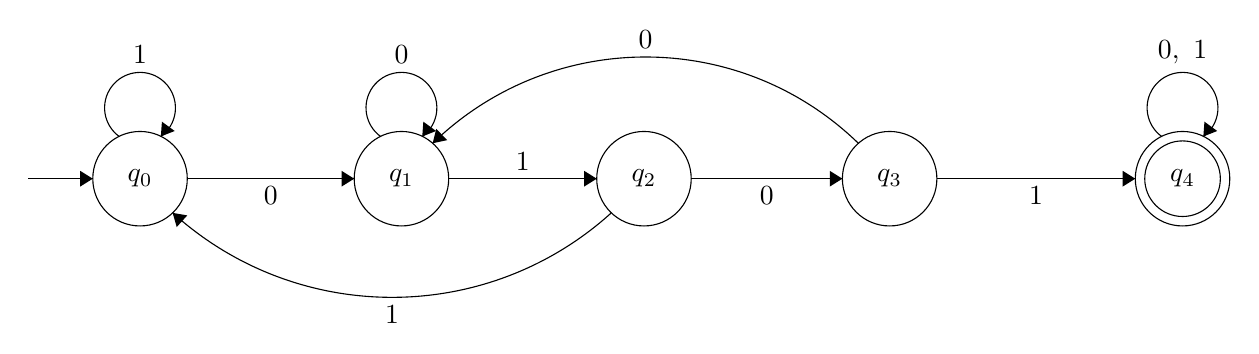
\begin{tikzpicture}[scale=0.2]
    \tikzstyle{every node}+=[inner sep=0pt]
    \draw [black] (7.9,-19.1) circle (3);
    \draw (7.9,-19.1) node {$q_0$};
    \draw [black] (24.5,-19.1) circle (3);
    \draw (24.5,-19.1) node {$q_1$};
    \draw [black] (39.9,-19.1) circle (3);
    \draw (39.9,-19.1) node {$q_2$};
    \draw [black] (55.5,-19.1) circle (3);
    \draw (55.5,-19.1) node {$q_3$};
    \draw [black] (74.1,-19.1) circle (3);
    \draw (74.1,-19.1) node {$q_4$};
    \draw [black] (74.1,-19.1) circle (2.4);
    \draw [black] (0.8,-19.1) -- (4.9,-19.1);
    \fill [black] (4.9,-19.1) -- (4.1,-18.6) -- (4.1,-19.6);
    \draw [black] (10.9,-19.1) -- (21.5,-19.1);
    \fill [black] (21.5,-19.1) -- (20.7,-18.6) -- (20.7,-19.6);
    \draw (16.2,-19.6) node [below] {$0$};
    \draw [black] (27.5,-19.1) -- (36.9,-19.1);
    \fill [black] (36.9,-19.1) -- (36.1,-18.6) -- (36.1,-19.6);
    \draw (32.2,-18.6) node [above] {$1$};
    \draw [black] (42.9,-19.1) -- (52.5,-19.1);
    \fill [black] (52.5,-19.1) -- (51.7,-18.6) -- (51.7,-19.6);
    \draw (47.7,-19.6) node [below] {$0$};
    \draw [black] (58.5,-19.1) -- (71.1,-19.1);
    \fill [black] (71.1,-19.1) -- (70.3,-18.6) -- (70.3,-19.6);
    \draw (64.8,-19.6) node [below] {$1$};
    \draw [black] (6.577,-16.42) arc (234:-54:2.25);
    \draw (7.9,-11.85) node [above] {$1$};
    \fill [black] (9.22,-16.42) -- (10.1,-16.07) -- (9.29,-15.48);
    \draw [black] (23.177,-16.42) arc (234:-54:2.25);
    \draw (24.5,-11.85) node [above] {$0$};
    \fill [black] (25.82,-16.42) -- (26.7,-16.07) -- (25.89,-15.48);
    \draw [black] (26.483,-16.853) arc (134.14834:45.85166:19.407);
    \fill [black] (26.48,-16.85) -- (27.41,-16.65) -- (26.71,-15.94);
    \draw (40,-10.87) node [above] {$0$};
    \draw [black] (37.829,-21.267) arc (-47.84822:-132.15178:20.755);
    \fill [black] (9.97,-21.27) -- (10.23,-22.17) -- (10.9,-21.43);
    \draw (23.9,-27.13) node [below] {$1$};
    \draw [black] (72.777,-16.42) arc (234:-54:2.25);
    \draw (74.1,-11.85) node [above] {$0,\mbox{ }1$};
    \fill [black] (75.42,-16.42) -- (76.3,-16.07) -- (75.49,-15.48);
\end{tikzpicture}
\caption{Diagrama de estados do AFD $M$ que reconhece $A$.}
\label{fig:sip1.6c}
\end{figure}

Agora, precisamos mostrar que o AFD $M$ reconhece a linguagem $A$, ou seja, para todo $w \in \Sigma^*$, $w \in L(M) \iff w \in A$.

Sem perda de generalidade, vamos assumir que $w$ é da forma $au$. Vamos definir $\forall w \in \Sigma^*$:
\begin{align*}
\deltaM(q_0, w) = \begin{cases}
                    q_0, \quad \text{se}\ w = \epsilon \\
                    \delta(q_0, w), \quad \text{se}\ w \in \Sigma \\
                    \hat{\delta}_M(q, u), \quad \text{se}\ w = au
                  \end{cases}
\end{align*}
\begin{align*}
    \text{onde} \ a \in \Sigma, |u| > 0 \ \text{e} \ q = \delta(q_0, a).
\end{align*}

Note que $\delta(q_0, w) = q \iff w \in L(q)$, ou seja, o autômato termina em um estado $q$ dado uma cadeia $w$, se e somente se, $w$ satisfaz as propriedades para o estado $q$. Sendo assim, vamos definir:
\begin{itemize}[label={}]
    \item $L(q_0) = $ \{$w \in \Sigma^* \ |\ $ 0101 não é subcadeia de $w$ e $w$ não termina com 0, 01 ou 010.\}
    \item $L(q_1) = $ \{$w \in \Sigma^* \ |\ $ 0101 não é subcadeia de $w$ e $w$ não termina com 01 ou 010, mas termina com 0.\}
    \item $L(q_2) = $ \{$w \in \Sigma^* \ |\ $ 0101 não é subcadeia de $w$ e $w$ não termina com 010, mas termina com 01.\}
    \item $L(q_3) = $ \{$w \in \Sigma^* \ |\ $ 0101 não é subcadeia de $w$, mas $w$ termina com 010.\}
    \item $L(q_4) = $ \{$w \in \Sigma^* \ |\ $ 0101 é subcadeia de $w$.\}
\end{itemize}

\textsc{Afirmação:} $L(M) = \{w \in \Sigma^* \ |\ w$ possui $0101$ por subcadeia\}, de forma tal que as propriedades (a), (b), (c), (d) e (e) valem $\forall w \in \Sigma^*$:
\begin{enumerate}[label=(\alph*)]
    \item $\deltaM(q_0, w) = q_0 \iff w \in L(q_0)$,
    \item $\deltaM(q_0, w) = q_1 \iff w \in L(q_1)$,
    \item $\deltaM(q_0, w) = q_2 \iff w \in L(q_2)$,
    \item $\deltaM(q_0, w) = q_3 \iff w \in L(q_3)$ e
    \item $\deltaM(q_0, w) = q_4 \iff w \in L(q_4)$.
\end{enumerate}

\begin{proof} Vamos provar a afirmação por indução em $|w|$.

\indbase $|w| = 0$\\[3pt]
Nesse caso, $w = \epsilon$ e, pela definição de $\deltaM$, temos que $\deltaM(q_0, w) = q_0$ e, portanto, $w \in L(q_0)$.\\
Por outro lado, se $w \in L(q_0)$, então, pela mesma definição de $\deltaM$, temos que $\deltaM(q_0, w) = q_0$.

\indhypo Suponha que a afirmação é verdadeira para qualquer cadeia $w$, tal que $|w| < n$.

\indstep Seja $w \in \Sigma^*$ e $|w| = n$. Lembrando que $w = au$, $a \in \Sigma$, $|u| > 0$ e $u \in \Sigma^{n - 1}$.

Agora, precisamos mostrar que a afirmação também vale para todas as possibilidades de transição de $\deltaM(q_0, u)$ e $a$.

\begin{enumerate}[label=\textbf{(\arabic*)}]
\item $\deltaM(q_0, u) = q_0$ e $a = 1$\\
Temos que $|u| < n$ e, por hipótese de indução, podemos concluir que $\deltaM(q_0, u) = q_0 \iff u \in L(q_0)$. Logo:
\begin{align*}
    \deltaM(q_0, w) &= \deltaM(q_0, au)\\
                    &= \delta(\deltaM(q_0, u), a)\\
                    &= \delta(q_0, a)\\
                    &= q_0
\end{align*}
Portanto, $\deltaM(q_0, w) = q_0 \iff w \in L(q_0)$.
%%%%%%%%%%%%%%%%%%%%%%%%%%%

\item $\deltaM(q_0, u) = q_0$ e $a = 0$\\
Temos que $|u| < n$ e, por hipótese de indução, podemos concluir que $\deltaM(q_0, u) = q_0 \iff u \in L(q_0)$. Logo:
\begin{align*}
    \deltaM(q_0, w) &= \deltaM(q_0, au)\\
                    &= \delta(\deltaM(q_0, u), a)\\
                    &= \delta(q_0, a)\\
                    &= q_1
\end{align*}
Portanto, $\deltaM(q_0, w) = q_1 \iff w \in L(q_1)$.
%%%%%%%%%%%%%%%%%%%%%%%%%%%

\item $\deltaM(q_0, u) = q_1$ e $a = 0$\\
Temos que $|u| < n$ e, por hipótese de indução, podemos concluir que $\deltaM(q_0, u) = q_1 \iff u \in L(q_1)$. Logo:
\begin{align*}
    \deltaM(q_0, w) &= \deltaM(q_0, au)\\
                    &= \delta(\deltaM(q_0, u), a)\\
                    &= \delta(q_1, a)\\
                    &= q_1
\end{align*}
Portanto, $\deltaM(q_0, w) = q_1 \iff w \in L(q_1)$.
%%%%%%%%%%%%%%%%%%%%%%%%%%%

\item $\deltaM(q_0, u) = q_1$ e $a = 1$\\
Temos que $|u| < n$ e, por hipótese de indução, podemos concluir que $\deltaM(q_0, u) = q_1 \iff u \in L(q_1)$. Logo:
\begin{align*}
    \deltaM(q_0, w) &= \deltaM(q_0, au)\\
                    &= \delta(\deltaM(q_0, u), a)\\
                    &= \delta(q_1, a)\\
                    &= q_2
\end{align*}
Portanto, $\deltaM(q_0, w) = q_2 \iff w \in L(q_2)$.
%%%%%%%%%%%%%%%%%%%%%%%%%%%

\item $\deltaM(q_0, u) = q_2$ e $a = 0$\\
Temos que $|u| < n$ e, por hipótese de indução, podemos concluir que $\deltaM(q_0, u) = q_2 \iff u \in L(q_2)$. Logo:
\begin{align*}
    \deltaM(q_0, w) &= \deltaM(q_0, au)\\
                    &= \delta(\deltaM(q_0, u), a)\\
                    &= \delta(q_2, a)\\
                    &= q_3
\end{align*}
Portanto, $\deltaM(q_0, w) = q_3 \iff w \in L(q_3)$.
%%%%%%%%%%%%%%%%%%%%%%%%%%%

\item $\deltaM(q_0, u) = q_2$ e $a = 1$\\
Temos que $|u| < n$ e, por hipótese de indução, podemos concluir que $\deltaM(q_0, u) = q_2 \iff u \in L(q_2)$. Logo:
\begin{align*}
    \deltaM(q_0, w) &= \deltaM(q_0, au)\\
                    &= \delta(\deltaM(q_0, u), a)\\
                    &= \delta(q_2, a)\\
                    &= q_0
\end{align*}
Portanto, $\deltaM(q_0, w) = q_0 \iff w \in L(q_0)$.
%%%%%%%%%%%%%%%%%%%%%%%%%%%

\item $\deltaM(q_0, u) = q_3$ e $a = 0$\\
Temos que $|u| < n$ e, por hipótese de indução, podemos concluir que $\deltaM(q_0, u) = q_3 \iff u \in L(q_3)$. Logo:
\begin{align*}
    \deltaM(q_0, w) &= \deltaM(q_0, au)\\
                    &= \delta(\deltaM(q_0, u), a)\\
                    &= \delta(q_3, a)\\
                    &= q_1
\end{align*}
Portanto, $\deltaM(q_0, w) = q_1 \iff w \in L(q_1)$.
%%%%%%%%%%%%%%%%%%%%%%%%%%%

\item $\deltaM(q_0, u) = q_3$ e $a = 1$\\
Temos que $|u| < n$ e, por hipótese de indução, podemos concluir que $\deltaM(q_0, u) = q_3 \iff u \in L(q_3)$. Logo:
\begin{align*}
    \deltaM(q_0, w) &= \deltaM(q_0, au)\\
                    &= \delta(\deltaM(q_0, u), a)\\
                    &= \delta(q_3, a)\\
                    &= q_4
\end{align*}
Portanto, $\deltaM(q_0, w) = q_4 \iff w \in L(q_4)$.
%%%%%%%%%%%%%%%%%%%%%%%%%%%

\item $\deltaM(q_0, u) = q_4$ e $a = 0$ ou $a = 1$\\
Esse caso é trivialmente verdade pois, nesse ponto, já sabemos que $u$ contém a subcadeia 0101 e, não importa o símbolo $a$ lido, temos que $\deltaM(q_0, u) = q_4 \iff u \in L(q_4)$ e $\deltaM(q_0, w) = q_4 \iff w \in L(q_4)$.
\end{enumerate}

Sendo assim, podemos concluir que o autômato $M$ da Figura \ref{fig:sip1.6c} está correto, pois $\deltaM(q_0, w) \cap F \neq \emptyset \iff w \in A$.
\end{proof}
